%  article.tex (Version 3.3, released 19 January 2008)
%  Article to demonstrate format for SPIE Proceedings
%  Special instructions are included in this file after the
%  symbol %>>>>
%  Numerous commands are commented out, but included to show how
%  to effect various options, e.g., to print page numbers, etc.
%  This LaTeX source file is composed for LaTeX2e.

%  The following commands have been added in the SPIE class
%  file (spie.cls) and will not be understood in other classes:
%  \supit{}, \authorinfo{}, \skiplinehalf, \keywords{}
%  The bibliography style file is called spiebib.bst,
%  which replaces the standard style unstr.bst.

\documentclass[]{spie}  %>>> use for US letter paper
%%\documentclass[a4paper]{spie}  %>>> use this instead for A4 paper
%%\documentclass[nocompress]{spie}  %>>> to avoid compression of citations
%% \addtolength{\voffset}{9mm}   %>>> moves text field down
%% \renewcommand{\baselinestretch}{1.65}   %>>> 1.65 for double spacing, 1.25 for 1.5 spacing
%  The following command loads a graphics package to include images
%  in the document. It may be necessary to specify a DVI driver option,
%  e.g., [dvips], but that may be inappropriate for some LaTeX
%  installations.
\usepackage{graphicx}

\title{Setting the standard: 25 years of operating the JCMT}

%>>>> The author is responsible for formatting the
%  author list and their institutions.  Use  \skiplinehalf
%  to separate author list from addresses and between each address.
%  The correspondence between each author and his/her address
%  can be indicated with a superscript in italics,
%  which is easily obtained with \supit{}.

\author{Jessica T Dempsey\supit{a}, Tim Jenness\supit{b}, Frossie Economou,\supit{c}, Remo P. J. Tilanus,\supit{d}, Antonio Chrysostomou,\supit{e}, Gary R. Davis\supit{a}, Holly S. Thomas\supit{a}, Craig A. Walther\supit{a}, Iain M. Coulson\supit{a}, Doug Johnstone\supit{a}, Per Friberg\supit{a}, Graham S. Bell\supit{a}\skiplinehalf
\supit{a}Joint Astronomy Centre, 660 N Aohoku Place, Hilo, USA \\
\supit{b}Cornell University, USA\\
\supit{c} National Optical Astronomy Observatory, USA\\
\supit{d} Netherlans Organisation for Scientific Research, Netherlands\\
\supit{e} University of Hertfordshire, UK\\
}

%>>>> Further information about the authors, other than their
%  institution and addresses, should be included as a footnote,
%  which is facilitated by the \authorinfo{} command.

\authorinfo{Further author information: (Send correspondence to J.T.D.)\\J.T.D.: E-mail: j.dempsey@jach.hawaii.edu, Telephone: 1 808 640 4243\\ }
%%>>>> when using amstex, you need to use @@ instead of @


\newcommand{\mnras}{MNRAS}
\newcommand{\procspie}{Proc.\ SPIE}
\newcommand{\aspconf}{ASP Conf.\ Ser.}

%%%%%%%%%%%%%%%%%%%%%%%%%%%%%%%%%%%%%%%%%%%%%%%%%%%%%%%%%%%%%
%>>>> uncomment following for page numbers
% \pagestyle{plain}
%>>>> uncomment following to start page numbering at 301
%\setcounter{page}{301}

  \begin{document}
  \maketitle

%%%%%%%%%%%%%%%%%%%%%%%%%%%%%%%%%%%%%%%%%%%%%%%%%%%%%%%%%%%%%
\begin{abstract}
  The James Clerk Maxwell Telescope (JCMT) is the largest single-dish
  submillimetre telescope in the world, and throughout its lifetime
  the volume and impact of its science output have steadily
  increased. A key factor for this continuing productivity is an
  ever-evolving approach to optimising operations, data acquisition,
  and science product pipelines and archives. The JCMT was one of the
  first common-user telescopes to adopt flexible scheduling in 2003,
  and its impact over a decade of observing will be presented.  The
  introduction of an advanced data-reduction pipeline played an
  integral role, both for fast real-time reduction during observing,
  and for science-grade reduction in support of individual projects,
  legacy surveys, and the JCMT Science Archive. More recently, these
  foundations have facilitated the commencement of remote observing in
  addition to traditional on-site operations to further increase
  on-sky science time. The contribution of highly-trained and engaged
  operators, support and technical staff to efficient operations will
  be described. The long-term returns of this evolution are presented
  here, noting they were achieved in face of external pressures for
  leaner operating budgets and reduced staffing levels. In an era when
  visiting observers are being phased out of many observatories, we
  argue that maintaining a critical level of observer participation is
  vital to improving and maintaining scientific productivity and
  facility longevity.
\end{abstract}

%>>>> Include a list of keywords after the abstract

\keywords{}

%%%%%%%%%%%%%%%%%%%%%%%%%%%%%%%%%%%%%%%%%%%%%%%%%%%%%%%%%%%%%
\section{INTRODUCTION}
\label{sec:intro}

The James Clerk Maxwell Telescope (JCMT) is the world's largest
single-dish submillimeter telescope. In operation since 1987, SCUBA-2
has only increased its scientific output and impact as the years have
passed. The reason for the continued relevance of the JCMT throughout
this time is partially the result of an ever-evolving and improving
instrument suite which has continued to break new ground in
submillimeter astronomy, from UKT14~\cite{1990MNRAS.243..126D} to SCUBA \cite{holland1999}
and now SCUBA-2\cite{holland2013}, as well as the 16-element heterodyne
HARP array\cite{buckle} and its backend ACSIS\cite{2000SPIE.4015..114H}. Another key
reason for this productivity has been the design and implementation of
flexible scheduling\cite{1998SPIE.3349..126W,tilanus2000,robson2002}, and the Observation
Management Project (OMP)\cite{economou2002}.  In 2014, the JCMT now
has over ten years of detailed performance metrics since the OMP was
fully implemented (flexible scheduing having been introduced some
years prior to that), and it can perhaps provide some insight into the
impact of these initiatives and provide some lessons for future
observation management.


%%%%%%%%%%%%%%%%%%%%%%%%%%%%%%%%%%%%%%%%%%%%%%%%%%%%%%%%%%%%%
\section{OBSERVING AT JCMT}

The JCMT currently operates a 12-hour single-shift observing night. A
Telescope System Specialist (TSS) is present at the summit, along with
a visiting observer. The observing cycle consists of two semesters
(Feb-July) and (Aug-Jan), for which up to 2013, the three partner
countries, the United Kingdom (60$\%$) Canada (20$\%$) and the
Netherlands(20$\%$) had separate time allocation committies (TACs) to
which observers from those countries would submit project
proposals. After the withdrawal of the Netherlands in 2013, the
process continued with the remaining partner countries. The JCMT has
operated a flexibly-scheduled observing queue for nearly fifteen
years. Observing blocks are allocated to each country queue, and the
TACs provide priority scheduling rules to determine the selection of
projects given weather conditions, availability and priority.

Flexible scheduling imposes as series of demands on the operation of
the telescope in order to ensure efficiency and high-quality data
output. Weather information must be known to a high-quality and
high-time-resolution, the telescope software interfaces with the
instruments and observing must be seamless and efficient,
instrument-switching should be fast in order to reduce down-time and
increase flexibility in changing weather conditions, and the observing
and reduction software should allow a tight feedback loop for the TSS
and observer to monitor data quality. Finally, this information should
be swiftly available to a P.I. who may not be present at the telescope
during their observations, in order to ensure their project is
completed as they require.

In addition to P.I. projects submitted to the TACs, the JCMT has
initiated a series of JCMT Legacy Surveys (JLS) with the introduction
of the two wide-field array instruments, HARP and SCUBA-2. These
surveys were started in 2007, after HARP was commissioned on the
telescope, with the SCUBA-2 components of the surveys starting in
2011. When it became clear that the JCMT would not continue operating
past September 2014, it was recognised that it would be a considerable
challenge to complete these surveys in the remaining time. It was felt
that allowing P.I. projects on the telescope was still an important
driver for the JCMT, but the survey allocations were increased to
60$\%$ of the available time in order to improve completion
potential. To further improve JLS completion, a new observing mode of
'Extended Observing', or partial remote operations from the JAC in
Hilo was added in early 2014. This mode and its impact is discussed in
Section~\ref{sec:eo}.

\subsection{JCMT Weather Grades}

Dynamic, or flexible, scheduling proposes to optimise the amount of
high-quality science observations completed by flexibly selecting
observations that are most appropriate for the conditions (weather and
source availability), and any other set of requirements (such as a
TAC-imposed project priority) that the Observatory may determine is
desired. \cite{tilanus2000} discusses the considerations for
scheduling that were initially taken by the JCMT upon the first
implementation of flexible scheduling in the late 1990s.

At submilimeter wavelengths, the appropriateness of queuing a given
project is defined first and foremost by the atmospheric opacity due
to water vapour. The transmission properties of the atmosphere above
Mauna Kea and their application to JCMT instruments and flexible
scheduling are described in detail elsewhere (\cite{robson2002}). A
linear relation exists between the measurable precipitable water
vapour (PWV) in mm and the opacity at the JCMT instrument
wavebands. This PWV is measured both by the adjacent CSO radiometer at
225GHz and an in-cabin line-of-sight 183GHz radiometer\cite{wiedner}),
allowing the atmospheric conditions to be measured at high
time-resolution. To allow for practical assessment of atmospheric
conditions, the PWV in mm is divided up into five weather 'bands' or
grades, and it is these grades that dictate the first-level scheduling
constraints for a given project.

\begin{table}
\caption{JCMT Weather Grades used for Project Selection. This table is an updated version of a table provided by \cite{robson2002}.}
\label{tab:grades}
\begin{center}
\begin{tabular}{|c|c|c|c|c|c|}
\hline
\rule[-1ex]{0pt}{3.5ex}  Grade & PWV(mm) & CSO 225GHz $\tau_{zen}$ & 850$\mu$m $\tau_{zen}$ & 450$\mu$m $\tau_{zen}$ & Notes  \\
\hline
\rule[-1ex]{0pt}{3.5ex}  1 & $< 1$ & $\tau<0.05$ & $> 82\%$ &   $ > 28\%$& Super dry, shortest $\lambda$ projects\\&&&&& that require highest senstivity\\
\hline
\rule[-1ex]{0pt}{3.5ex}  2 & $1.0 < 1.6$ & $0.05<\tau<0.08$ &  $ \approx77\%$ & $\approx19\%$ &Very dry, high sensitivtity 850$\mu$m projects\\&&&&& and 450$\mu$m spectroscopy\\
\hline
\rule[-1ex]{0pt}{3.5ex}  3 & $1.6 < 2.4$  & $0.08<\tau<0.12$ &  $\approx67\%$ & $\approx7\%$ & Dry, brighter 850$\mu$m targets\\ &&&&&(eg. large-scale galactic surveys)\\
\hline
\rule[-1ex]{0pt}{3.5ex}  4 & $2.4 < 4.0$ & $0.12<\tau<0.2$ &  $\approx53\%$ & $\approx2\%$ & Poor: long $\lambda$ spectroscopy \\&&&&&and bright 345GHz surveys\\
\hline
\rule[-1ex]{0pt}{3.5ex}  5 & $ > 4.0 $ & $0.2<\tau$ & $ < 45\%$ & $< 0.5\%$&  Wet: spectroscopy at $\lambda > 850 \mu$m \\
\hline

\end{tabular}
\end{center}
\end{table}

As the opacity increases, more time is required on sky to reach the
same sensitivity at a given wavelength. The transmission varies
strongly with observation wavelength. The 450$\mu$m atmospheric window
requires much dryer conditions to be an effective observing
band. Table~\ref{tab:grades} reproduces a similar table by
\cite{robson2002} which describes the properties of each grade and the
relevant transmission properties at the main SCUBA-2 filter
bands. Figure~\ref{fig:tau} collates the typical percentage of time
each month that the opacity is measured in a particular band, averaged
over nightly measurements taken every night from 2003 to 2014.

  \begin{figure}[h]
   \begin{center}
   \begin{tabular}{c}
   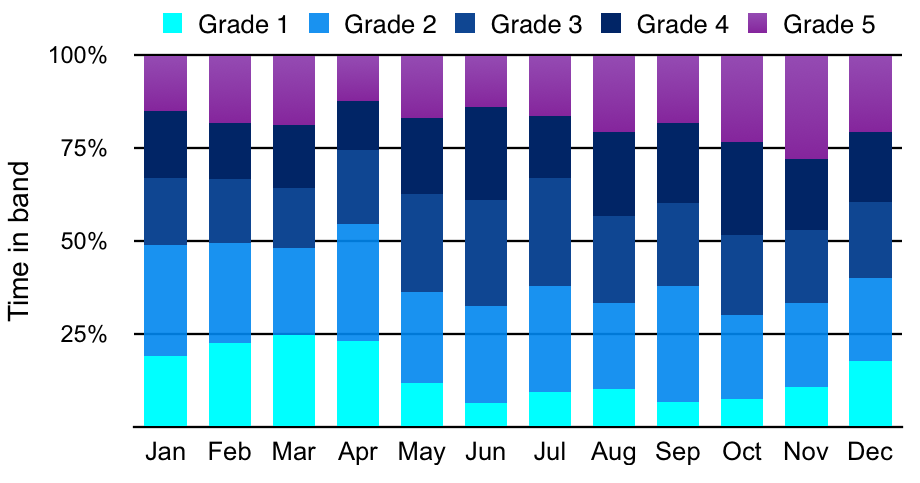
\includegraphics[height=5cm]{tauaverageperc.png}
   \end{tabular}
   \end{center}
   \caption{\label{fig:tau} Percentage of available observing time in weather Grades 1 through 5, averaged by month over measurements taken nightly between 2003 and 2014 .}
\end{figure}

\subsection{Project Priority}
In the automated queue, potential observations are selected, and then
ordered, by the following parameters:
\begin{itemize}
\item The current zenith opacity (and thus weather Grade)
\item The observation length and object availability
\item The project priority as allocated by the Time Allocation Committee (TAC)
\end{itemize}

A good deal of discussion has occurred regarding the most effective
methodology for determining project priority and how it translates to
project completion and scientific impact\cite{adamson2004,robson2002}.
In practice, the case at JCMT was further complicated by the fact that
the facility was funded jointly by the UK (60$\%$), Canada and the
Netherlands (20$\%$ each) and thus were allocated the respective
amount of telescope time as a result. The countries had separate TACs,
and thus it was left to each TAC to determine their own flexible
scheduling rules for their allocated blocks as well as how many
projects to award time to and how to prioritise them.

\section{Instrument and Telescope interfaces}\label{sec:inst}

In order to take full advantage of the benefits of flexible
scheduling, there have been adaptations in instrument design, and
observatory software systems. The ability to switch swiftly between
instruments is perhaps the most powerful of these. The current
instrument suite consists of three heterodyne receivers, HARP
(345GHz), RxW (690GHz) and RxA (230GHz) and the continuum camera,
SCUBA-2 (simultaneous 450$\mu$m and 850$\mu$m). Including pointing,
focus and instrument setup times, it takes less than fifteen minutes
to swtich from a completed observation with one instrument to the
first science observation with another. The critical developments
required to allow this include a rotating tertiary mirror in the
cabin, and a sophisticated telescope software interface between the
telescope, instruments and observer [REFERENCE- craig]. It has also
been a requirement that any instrument commissioned at JCMT must
support this shared operational and data-reduction software to
maintain the efficiency of these observing interfaces. Fast-switching
between instruments has the added benefit of reducing 'dead-time'
resulting from instrument-related faults, as a time-consuming issue
with a particular instrument can be dealt with after switching to a
working instrument, which can continue to take data whilst the
original problem is resolved.



\section{The OMP}\label{sec:omp}

Arguments against flexible scheduling often highlight the concern that
PIs are removed from adapting and assessing the quality of their
observations in a flexible regime, and that an observer present at the
telescope may have neither the skills or interest in providing such
assessment on the time-scales needed to ensure good data
quality. Thus, as noted by \cite{tilanus2000}, a tight feedback loop
between the Observatory and PI is necessary. Additionally, there is a
need to provide general and well-documented quality assessment tools
at the telescope to aid inexperienced or differently-skilled observers
in data monitoring. The concept for an overarching OMP that supported
both the JCMT and UKIRT observing was developed to provide an
observation preparation tool for PIs, a tool to query the database
given the weather constraints and priority as defined by the given
country queue rules, an extensive database-generated set of web pages
to alow the PI to assess project completion, quality and to retrieve
data files, and a method for support astronomers to communicate with
PIs to give feedback and adaptations on observing plans. Details of
the OMP can be seen in \cite{2011tfa..confE..42J}.

The OMP provides a comprehensive feedback system which automatically
logs project completion, observations, nightly conditions and faults
occurring, as well as a detailed commentary of the night's observing
progress. The fault system is an example of the ways in which
automated accounting and feedback improve observatory performance. An
example search of the JCMT fault system is shown in
Figure~\ref{fig:faulteg}. It can be seen that faults fall into
specific categories based on system (eg SCUBA-2), type (eg
electronic), current status, and time lost. The observer will be
notified if a fault potentially affected their data, and be able to
seek JCMT support staff assistance if there is a concern. The fault
system's true power lies in the database of previously faults that
telescope support staff, engineers and operators can use to
troubleshoot existing and reocurring issues and also as a teaching
tool. Finally, the tracking of time lost due to individual faults
provides a tight feedback loop in prioritising those issues which have
the greatest impact on observing efficiency and quality.

 \begin{figure}[ht]
   \begin{center}
   \begin{tabular}{c}
   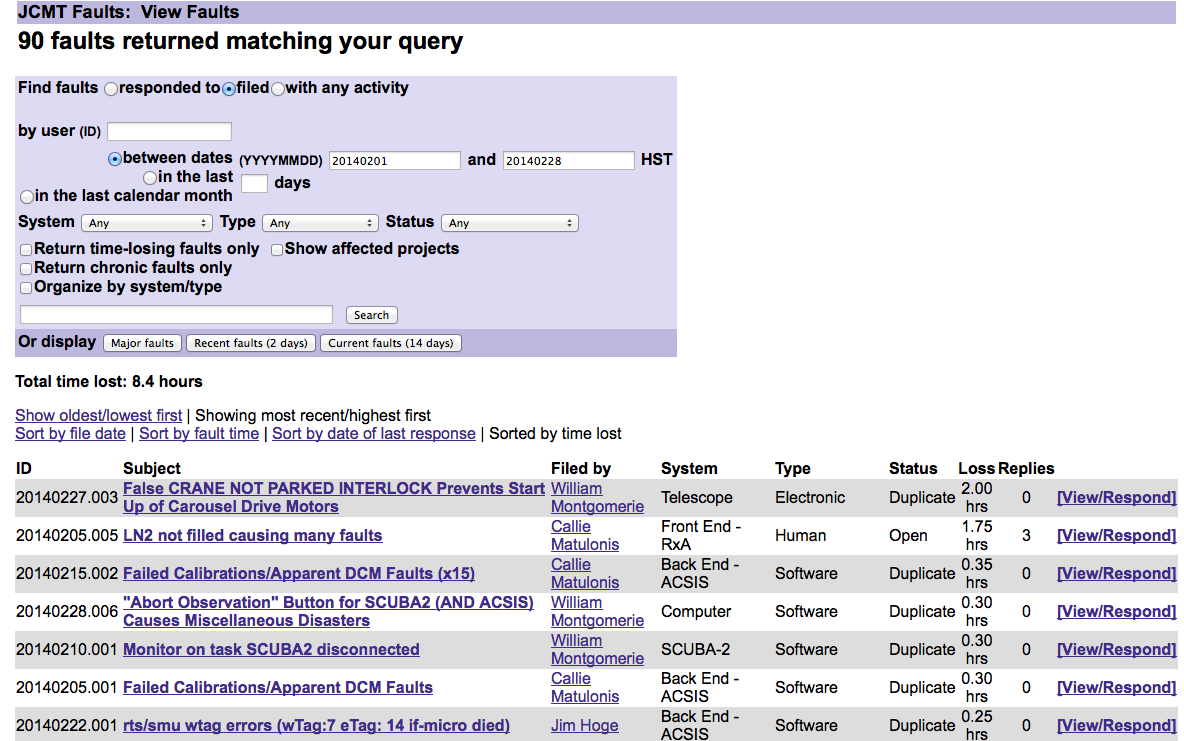
\includegraphics[height=10cm]{faultexample.png}
   \end{tabular}
   \end{center}
   \caption{\label{fig:faulteg}Example search of the OMP fault system.}
\end{figure}


\section{PERFORMANCE METRICS} \label{sec:metrics}

There are a number of metrics that the JCMT monitors on a weekly,
monthly and semester-basis to track the telescope performance and
efficiency. Nearly all of the data presented here is found in the OMP
database, making comparison and tracking relatively simple. It is
interesting to note that project time measured on a weekly and monthly
basis shows very little variation in the ten years since monitoring
began. In 2006, JCMT switched from a two-shift, 16-hour observing
schedule to a single, 12-hour observing night. Whilst the 'on-sky'
project time dips understandably when this mode began, the advantage
lay in that the early-evening shift was systematically poorer in
observing conditions, and less high-quality data obtained as a
result. The difficulty lies in quantifying the impact of taking less,
but higher-quality data after this change was enacted.

Improvements in observing methodology, software efficiency and data
reduction and analysis have all improved the quality of JCMT data. At
the telescope, such improvements are driven by the feedback loop
provided by fault reporting from our TSS and observer to telescope and
support staff. This reporting is discussed in
Section~\ref{sec:rates}. With flexible-scheduling, the observatory
relies heavily on a well-trained TSS with experience in not just the
telescope operation and software but also has familiarity with the
science output of the instrument suite and be able to provide some
quality assessment during observing. At the JCMT, the TSS serves along
side the support astronomer in providing information to the visiting
observer regarding observing priorities, methodology and quality
assessment.

\subsection{Publications}
 \begin{figure}[ht]
   \begin{center}
   \begin{tabular}{c}
   \includegraphics[height=5cm]{JCMT_publications.png}
   \end{tabular}
   \end{center}
   \caption{\label{fig:pub} Publications per year at the JCMT between 1988 and the end of 2013.}
\end{figure}

The most accepted metric for telescope performance is the number of
publications from its science in each year. This is presented for the
JCMT in Figure~\ref{fig:pub}. The JCMT is the most successful
single-dish submillimeter telescope in the world and this is reflected
in its high output of papers. The bulk of these papers are from SCUBA
data - to the end of 2013 over 800 papers have been published from
SCUBA, over 50$\%$ of the entire publication output of the
telescope. One of the frustrations of using this metric is the long
delay between acquisiton of science data and the publication of its
results. The average is suggested to be approximately four years. As
such, at the end of 2013, 43 papers have been published using SCUBA-2
since it was fully commissioned in late 2010. The number per year
tripled from 6 to 18 between 2012 and 2013, however. If returning to
the comparison with SCUBA, which output 19 papers in 1998 , it would
suggest a potential further factor of three increase in the next year.


\subsection{Fault Rates}\label{sec:rates}

The JCMT board sets a requirement that the observatory maintain a
fault rate of less than 5$\%$. For 12-hour nightly shifts, this
equates to a approximately a half-hour of time-lost due to faults. The
JCMT fault-rate averaged on a monthly basis since February 2003 is
shown in Figure~\ref{fig:fault}. The figure serves to highlight the
benefit of tracking fault-rates in this manner. The consistently
higher fault periods can be directly correlated with instrument
commissioning - notably the period in late 2006 and early 2007 when
the HARP and ACSIS instruments were commencing operation. This fault
percentage is calculated with respect to 'clear-time' which first
deducts time lost to weather from the 12-hour available night. Thus a
ten-minute fault on a night with many hours lost to weather is
reflected as a higher percentage of that night's available time, as
opposed to the same fault on a night with no weather-imposed facility
closure.

 \begin{figure}
   \begin{center}
   \begin{tabular}{c}
   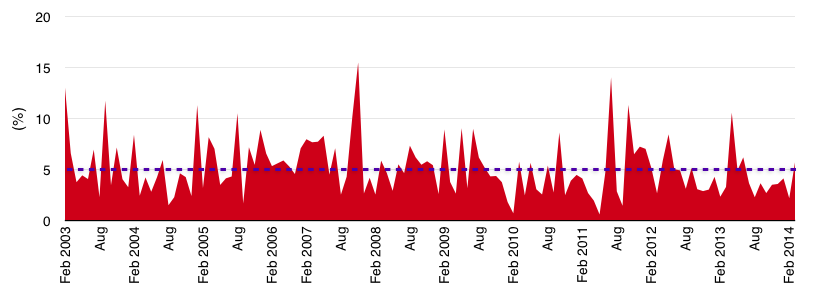
\includegraphics[height=3.5cm]{Faultrate2003_2014.png}
   \end{tabular}
   \end{center}
   \caption{\label{fig:fault}Monthly fault rate from the OMP fault reporting system since implementation (2003) until April 2014.}
\end{figure}

\subsection{Flexible versus Classical Scheduling}\label{sec:sched}

With reference to the JCMT, only anecdotal evidence has been used to
argue the benefits of flexible scheduling versus a classical regime.
In order to look at this more systematically, a direct comparison
between completion rates in a classical versus flexible regime is
needed. The detailed logging of project completion and other metrics
was only instigated with the advent of the OMP, when flexible
scheduling was already in place, so we lack sufficient classically
scheduled metrics for this comparison. Simulating this comparison
therefore required returning and 'classically-scheduling' two full
semesters of project time in January 2007 - January 2008. This was a
'blind' scheduling, in the sense that the scheduler was asked only to
take the project allocations and priorities given by the three TACs
for those semesters and allocate time to them according to the
proportions of time each country queue was allowed. The scheduler had
no other information regarding weather conditions, faults that
occurred during that year or any other information, so as best to
simulate what would occur prior to the start of any normal semester.

\begin{figure}[ht]
   \begin{center}
   \begin{tabular}{c}
   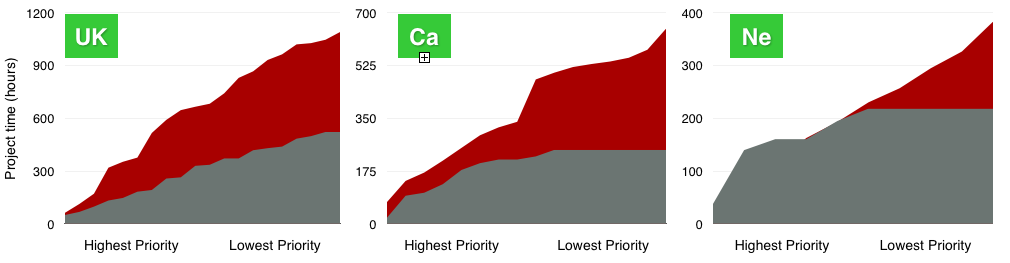
\includegraphics[height=3.5cm]{projecthours_cumul_2007.png}
   \end{tabular}
   \end{center}
   \caption{\label{fig:cvf_hours} Cumulative plot of the number of project hours completed as a function of project priority in the measured flexible scheduling case (red) and the simulated classical allocation (grey) for the United Kingdom (left), Canadian (centre) and Netherlands queues (right).  }

\end{figure}
\begin{figure}
   \begin{center}
   \begin{tabular}{c}
   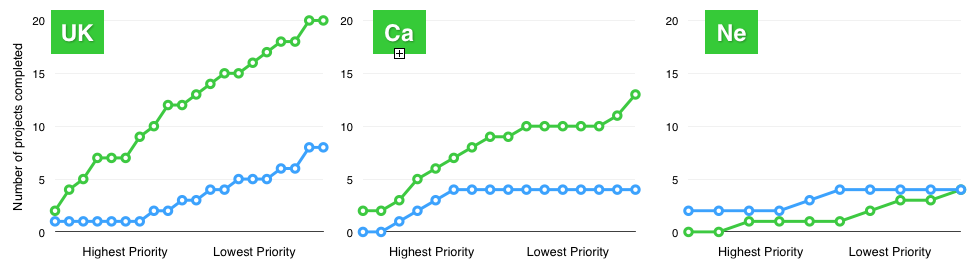
\includegraphics[height=3.5cm]{numprojcomp_cumul_2007.png}
   \end{tabular}
   \end{center}
   \caption{\label{fig:cvf_proj} Cumulative plot of the number of projects completed to better than 80$\%$ as a function of project priority for the measured flexible scheduling case (blue) and simulated classical allocation (green) for the  United Kingdom (left), Canadian (centre) and Netherlands queues (right).}
\end{figure}

The classical schedule was then taken and the known metrics from the
nights each project was allocated were used to estimate the amount of
time they would have received. The following assumptions were made:
\begin{itemize}
\item If the weather grade during the night was equal to or better
  than that required for the project, the project was allocated the
  full 'clear-time' available from that night (available time minus
  fault time).
\item If the weather grade was one grade 'poorer' than that required,
  the project was allocated half the time it would have obtained in
  its required grade.
\item If the weather was two or more grades poorer than required, no
  time was allocated.
\end{itemize}

Figure~\ref{fig:cvf_hours} presents the comparison between the
cumulative project hours for the actual, flexibly-scheduled projects,
and the same projects when scheduled classically as described
above. The cumulative plot is calculated as a function of priority,
with the highest-ranked projects to the left. Thus, if the projects
are scheduled to be completed as a function of priority, this plot
should rise steeply from the left, and flatten out towards the
lower-ranked projects. The grey cumulative area represents the
simulated classical hours as priority decreases, whilst the red
represents the measured cumulative project hours. The three country
allocations are presented separately, as indicated in the figure.

In total across all country queues, 60 projects were classically
scheduled, based on their requested time and priority and the time
available. In the flexible scheme, 92 projects were allocated time in
the year. It is noted that some TACs overfill their queue in a
flexible scheduling mode, and that also a number of these projects
were for small amounts of time, which would not have been as likely to
have been allocated time in a classical regime. In comparing directly
the same 60 projects that were scheduled in both the flexible and
classical regime, 1233 hours were observed in the flexible case,
compared to 986 hours in the classical queue. Of these, 25 projects
were completed to better than 80$\%$ of their requested time, compared
with 16 in the classical case. If one takes into account the
additional 32 projects that got some amount of time in the flexible
case, the additional hours observed takes the total project time
observed in the flexible case to 2117 hours and an additional 12
projects completed to better than 80$\%$.

Other notable results that are not shown in the figure include the
fact that in the flexible-schedule mode, more projects with small time
requirements can be reasonably scheduled. Projects that only require a
few hours of time, or perhaps have a source only observable for a
short period during a single night, would not likely be given time in
a classical scheduling regime, yet were able to be given time and
completed in a flexible queue. Finally, it is worth noting that four
projects in the classical simulation made their observations in
weather two or more grades better than they required. This could be
argued as poorly-used time, since projects needing the better weather
lost out in this scenario. A strong caveat to this comparison is that
the time allocation commitees would undoubtably have prioritized and
allocated time much differently if they were classically scheduling
their time.

\subsection{Sky Coverage with wide-field array instruments}

As stated previously, project hours do not necessarily correlate with
the scientific impact of observations. A single-dish telescope such as
JCMT holds great value in its capacity for wide-field, large-area
surveys in the era of ALMA and SKA. In both heterodyne and continuum,
the observatory has continued to lead the design and commissioning of
wider-field, high-speed and -sensitivity survey instruments to improve
sky coverage and depth. In the continuum, SCUBA (1997 - 2005) forged
the path for SCUBA-2 (2009 to present), and in the heterodyne, the
16-element 345GHz HARP (2007 to present) replaced the single-element
RxB receiver. In Figure~\ref{fig:sc2}, the cumulative sky coverage of
SCUBA and SCUBA-2 is plotted. The coverage is in square degrees of sky
and is presented on a logarithmic scale. This is because with the
advent of SCUBA-2, the increase in sky coverage over the total
observed with SCUBA, is a factor of nearly 50, after only three and a
half years of SCUBA-2 observing, increasing from the total coverage of
41 square degrees (SCUBA) to 2020 square degrees (SCUBA-2).

Figure~\ref{fig:het} shows the cumulative sky coverage acheived with
the heterodyne suite of instruments. To 2007, this consisted of
single-element receivers at three specific frequency bands. HARP, the
16-pixel array receiver, was commissioned in early 2007. Since 2007,
HARP has allowed an increase in sky coverage from 17 square degrees to
over 350 square degrees, a factor of 20 increase. It must be noted
that this sky coverage is at a range of frequencies, not simply
345GHz, and serves only to illustrate the power of array-receivers
over single-pixel elements. The analysis also does not describe the
sensitivity depth of the coverage, which varies and of-couse depends
entirely on the scientific goals of the observations.

\begin{figure}[h]
   \begin{center}
   \begin{tabular}{c}
   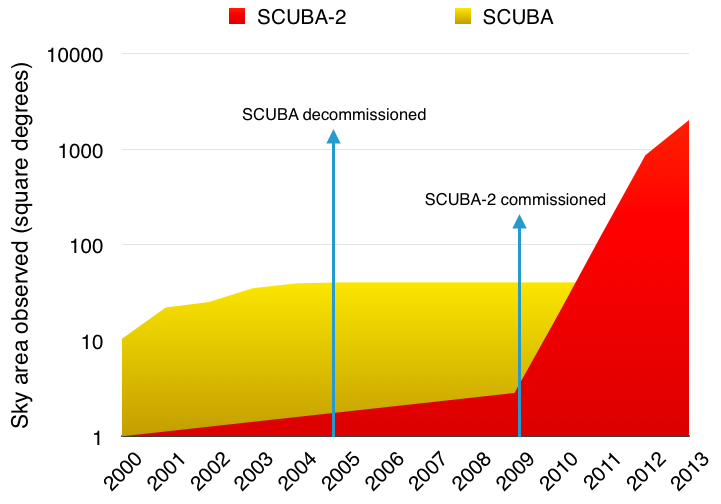
\includegraphics[height=5cm]{scuba2scuba_areacover.png}
   \end{tabular}
   \end{center}
   \caption{\label{fig:sc2} Plot of cumulative sky coverage of SCUBA (yellow) from 200 through to its decommissioning in 2005 and SCUBA-2 (red), commissioned in 2010. Coverage is in logarithmic square degrees.}
\end{figure}

\begin{figure}[h]
   \begin{center}
   \begin{tabular}{c}
   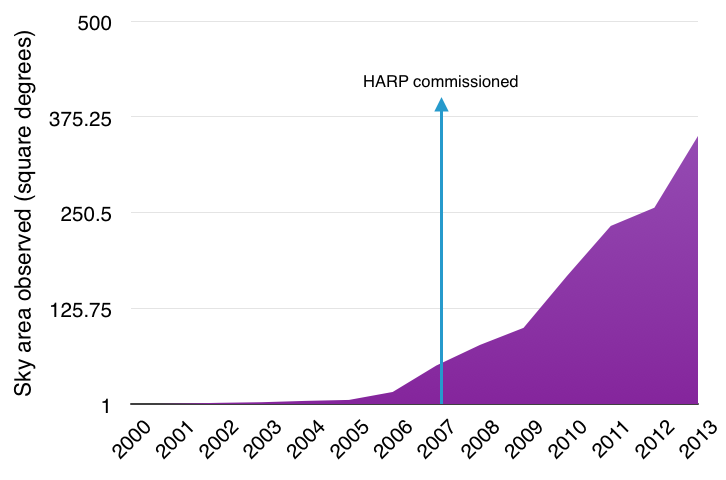
\includegraphics[height=5cm]{heterodyne_areacover.png}
   \end{tabular}
   \end{center}
   \caption{\label{fig:het} Plot of cumulative sky coverage for the combined heterodyne receivers. Whilst this does not separate the receivers specifically, the striking increase in late 2006 to the present indicates the operation of the HARP receiver since that time. Coverage is in logarithmic square degrees.}
\end{figure}

\subsection{The impact of Extended Observing}\label{sec:eo}


As previously mentioned, with only an average of less than half an
hour of fault loss per night, and consistent calibration rates of
approximately 25$\%$, the overall project time per night is extremely
consistent and affected primarily by any time lost to weather. As such
the only way of truly increasing project time is to extend operations
beyond the current 12-hour nightly shift. UKIRT shifted to fully
remote operations in 2012 [REFERENCE?]. This paved the way for JCMT to
incorporate remote observations to its observing program. Various
limitations prevented a shift to fully remote operations at the JCMT
and as such a mode was designed whereby at the end of the 12-hour
shift and prior to the arrival of the JCMT daycrew, operational
control is handed over from the summit operator and observer to a
remote operator at JACs Hilo facility. Four days a week, this
additional project time is between an 1.5 and 2.5 hours. Friday
through Sunday, when no daycrew are at the summit, this time extends
into the afternoon, and up to 5 hours of projects can be observed.

The highest priority for the JCMT in this time is the completion of
the JCMT Legacy Surveys with SCUBA-2. Thus, the extended observing
currently limits observing to just these programs. As such, it is
possible, knowing the average time extended observing gains, an
estimate of the increase in completion of the surveys can be
estimated. Figure~/ref{fig:eo} shows the increase in completion for
the surveys in total with and without extended observing. An
additional 8$\%$ completion can be acheived in only six months (a
total of XX hours) with the addition of this mode.

\begin{figure}[ht]
   \begin{center}
   \begin{tabular}{c}
   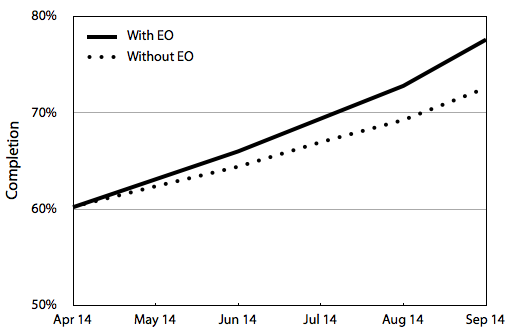
\includegraphics[height=5cm]{JLScompletion-SPIE.png}
   \end{tabular}
   \end{center}
   \caption{\label{fig:eo} Plot of predicted JLS completion up to September 2014 with extended observing (solid line) and without extended observing (dashed line).}
\end{figure}


\section{THE JCMT LEGACY}

The JCMT strives in its operations to continually optimise its
scientific output and impact. Over the course of 25 years of
operation, the legacy of scientific data that the facility has
produced will continue to provide scientfic value for decades to
come.n this paper, we have also demonstrated the tools and
methodologies that have been of use in maximising this science output
and include:
\begin{itemize}
\item Flexible scheduling to optimise use of available weather and
  maximise scientific project completion
\item Fast instrument switching to reduce dead-time and enhance
  redundancy
\item Detailed fault-reporting to optimise the feedback loop between
  the TSS and operational staff and minimise lost time
\item An advanced observing feedback interface (OMP) to enhance data
  delivery and quality information to the P.I. and observer
\item Highly trained operators to ensure data-quality and observing
  efficiency
\item Extended, remote operations to maximise project time
\end{itemize}

The JCMT legacy will be ensured by the continuing development of the
JCMT Science Archive,\cite{jsahistory} which will provide a searchable,
online database of all JCMT science data with advanced data-reduction
products and catalogues.\cite{2014SPIE9152-93}

%%%%%%%%%%%%%%%%%%%%%%%%%%%%%%%%%%%%%%%%%%%%%%%%%%%%%%%%%%%%%
\acknowledgments     %>>>> equivalent to \section*{ACKNOWLEDGMENTS}


%%%%%%%%%%%%%%%%%%%%%%%%%%%%%%%%%%%%%%%%%%%%%%%%%%%%%%%%%%%%%
%%%%% References %%%%%

\bibliography{9149-51}   %>>>> bibliography data in report.bib
\bibliographystyle{spiebib}   %>>>> makes bibtex use spiebib.bst

\end{document}
